\documentclass[twoside,headings,a4paper]{article}
\usepackage[Wingdings, OrigBox]{FlyingCircus}

\begin{document}

% SEt the document title, and you can add text at the bottom of the page.
% There's a \vfill pushing text to near the bottom, so you'll have to 
% manually create spacing from that.  Another \vfill is a convenient distance.
\InsertFCTitleAndTOC{\LaTeX{} Template}{
    Can add a Dedication
    \vfill
    Author Names
}

% The basic Aircraft function.
% You have to set the top few manually, but everything below that
% Can be copied from the Save Catalog button on the plane builder.
% Things left unset generally appear as giant purple boxes, like the
% Nickname does for this one.
% There's also a `Box Loc' variable that can be any of the points on the image
% north, north east, east... north west, center, ect.
\FCPlane[Nickname=\FrameDefault{Not Set}, %Box Text = {}, Image = {},
    Name={Basic Biplane}, Price=11, Used=5, Upkeep=0,
    Stats = {
            Full Load & 1 & 99 & 3 & 8 & 13 \\
            \nicefrac{1}{2}, Bombs & 1 & 100 & 4 & 6 & 13\\
            Full Fuel & 2 & 100 & 5 & 6 & 14\\
            Half Fuel & 2 & 100 & 5 & 5 & 14\\
            Empty & - & 101 & - & 5 & 0\\
        },
    Vital Parts = {Controls, Fuel Tanks, Engine \#1, Oil Tank \#1, Landing Gear},
    Crew = {Pilot},
    Propulsion = {Dropoff 8, Reliability -1, Overspeed 18, Ideal Alt. 0-29, Fuel 12},
    Aerodynamics = {Visibility -1, Stability -1, Energy Loss 3, Turn Bleed 1 (2)},
    Survivability = {Toughness 8, Max Strain 34, Escape 2, Crash Safety -1, Flight Stress 2},
    Armament = {5 Bomb Mass Externally. \\
            Seat \#1: 1x Fixed MG ✣ fires [Forward] for 2 damage with 4/3/2/1 hits with 10 ammunition. [Jam 2/3, Rapid Fire, AP 1, Fully Accessible]\\
            Rotary:  +1 to Dogfight! when turning right.\\
        },Link = {https://tetragramm.github.io/PlaneBuilder/index.html?json=AAEAjATAdArMCwAhAhgZwJYGMAEj0AcAbZAOwFNgBAK4WgMFsfqcZBfZoHQAlACwHsSybAFl+AF34AnAEbIArtgBaYMNgAcABl75gAJGABcYACBa1GkzYAIVhw4B-h8FsAoex8-ngPAUNES0nKKKmpaOsAAwADq0QCSPnyCwmKSsgrKqhraurRmlACCUABmxQACAAmMAJBUAPwAAbSNzU32bEwWTp5mHL1RXvb9PZ2mjLa2HhPskXaj3p6zNZaDy6ssAKCe1BZsFhxbXku0k+sD9gDgZ8fnZx7UkdR0+4w7++-3d19AA}
]{
    % This is where you put the text that goes between the bottom of the stats
    % And the Plane Builder Link.  It's a multi-column environment, so just use 
    % \columnbreak to go to the second column, or let it wrap by itself automatically.
}
\begin{tikzpicture}[remember picture, overlay]
    \node[text opacity=1, inner sep=0pt, outer sep=1cm, anchor=north east] at (image.north east) {
        \contourlength{1pt} %how thick each copy is
        \contour{black}{\textcolor{white}{\fontsize{50}{60}\Kochfont{}Bonus?}}
    };
\end{tikzpicture}

%Note that Price is empty.  This plane cannot be bought new, for flavor reasons.
% If Price, Used, or Both are empty, the appropriate sections will be missing.
\FCPlane[Name = Bergziegel, Image = {Bergziegel_image.png},
    Box Text = {
            Role & Transport\\
            First Flight & 1603\\
            Strengths & Room for Everything\\
            Weaknesses & Speed\\
        },
    Price = {}, Used = 8,
    Nickname = {Bring the bacon, and everything else!}, Upkeep = 2,
    Stats = {
            Full Load              & 1     & 87       & 1     & 6     & 11    \\
            \nicefrac{1}{2}, Bombs & 2     & 90       & 1     & 4     & 11    \\
            Full Fuel              & 2     & 91       & 1     & 4     & 11    \\
            Half Fuel              & 2     & 92       & 1     & 3     & 11    \\
            Empty                  & -     & 93       & -     & 3     & 0     \\
        },
    Vital Parts = {x2 Engines, x2 Oil Tanks, Controls, Fuel Tanks, Landing Gear},
    Crew = {Pilot},
    Propulsion = {Dropoff 6, Reliability -1/-1, Overspeed 20, Ideal Alt. 0-29, Fuel 7},
    Aerodynamics = {Visibility -1, Stability 4, Energy Loss 10, Turn Bleed 1 (2)},
    Survivability = {Toughness 11, Max Strain 20, Escape 2, Crash Safety -1, Flight Stress 2},
    Armament = {Passengers: 5 cabin seats and 0 first class or stretcher seats.\\
            Large Cargo: Will fit a scout or fighter aircraft with the wings taken off.},
    Link = {https://tetragramm.github.io/PlaneBuilder/index.html?json=AAEAjATAdArMBQAhApgJwOYC8CWz3IBtgBAE4cgMHOspupDvIFBzSAgYADACUALAewB2AQwAEAWX4AXfqgBGwgK6iAWpFFgwABl4AHYABRgAXGABgVpZpUAENQDgjJ8AD-L4AGhgABGd--ljwCIhLSsgrKahAa2nrmAOrxAJJcfEJikjLySqrqmjr65BzEAIKFAAIABdQAkCQA-AAyADMAs-UAAeSdfgw0pK7uVAHkQemhWRG50flxRqYWZEvUtg4j5G6ePus7gWkhmeE5UTEFCcmpwRlh2ZF5sYXAxWXkVbUNLe1dwD3OfdQDTbDXYcch1XYQyGMRaQmFkUHAACYCEYAyRKLoMLhyzRzjhdQRO3BkJYflIAwYhPW-3MNDsEOxNEcOzhjKhdFx7P8QA}
]{
    After the end, helping communities get in touch with those around them and restoring trade was one of the most important things.  Into the gap stepped the Baron, with the Bergziegel design.  This innovative transport could move people and large cargos as far as it's escorts could keep it safe.

    One of the cheapest large transports you'll ever find, this steady, reliable plane has traveled the skies of Himmilgard for more than 15 years.

    \columnbreak

    \begin{itemize}
        \item The external nacelle engine mounts can be modified to use nearly any type of engine, or even asymmetric engines while still being stable and easy to fly.
        \item Add extra fuel to travel long-distances.
        \item Trade cargo space for up to 15 additional passengers
        \item An extended fuselage can allow even huge cargos to be carried.
    \end{itemize}
}

% This is an example Vehicle function
% It always starts on the left page, because it forms
% a double page spread, so count your pages.
% The text is placed on the left page.
% Anything below the stat block on the right page just goes after this function.
% So, you know, just keep typing after the last bracket.
\FCVehicle[Name = What's A Tank?, Price = 30000,
    Nickname=The Worst Tank, Upkeep=200,
    Speed = 0, Torque = -0, Handling = 0,
    Armour = 0/0/0, Integrity = 0, Safety = 0,
    Reliability = 0, Fuel Uses = 0, %Stress = 1,
    Size = Huge Size, Cargo = Some Tiny Cargo,
    Crew = {
            Driver & Closed & 0 & 1 & Hatch \\
            Commander & Closed & 2 & 3 & Hatch \\
            Gunner & Closed & -1 & -2 & Big Gun \\
            Loader & Closed & -3 & -4 & \\
            x6 MG Crew & Closed & - & - & Guns?  Guns! \\
            Mechanic & Sealed & - & - & Engine Access \\
        },
    Box Text = {
            Year Introduced: 2023\\
            Served With: Rolling Circus\\
            Engine: Lua\LaTeX\\
            Strengths: Sophisticated\\
            Weaknesses: Complicated\\
            Inspiration: Erika Chappell\\
        },
    Facing Image = Wandelburg.png,
    Text Offset = -1.5cm
]{
    Lorem ipsum dolor sit amet, consectetur adipiscing elit, sed do eiusmod tempor incididunt ut labore et dolore magna aliqua. Volutpat commodo sed egestas egestas fringilla. Diam vel quam elementum pulvinar etiam non quam lacus suspendisse. Eget dolor morbi non arcu risus. Quis viverra nibh cras pulvinar mattis nunc sed blandit. Elementum tempus egestas sed sed risus pretium quam. Feugiat in ante metus dictum at tempor commodo ullamcorper a. Ultricies mi eget mauris pharetra et. Elementum nisi quis eleifend quam. Posuere urna nec tincidunt praesent semper feugiat. Amet nisl purus in mollis nunc sed. Sed arcu non odio euismod lacinia at quis. Mauris in aliquam sem fringilla ut morbi. Enim neque volutpat ac tincidunt vitae semper. Amet volutpat consequat mauris nunc. Fermentum posuere urna nec tincidunt praesent. In nulla posuere sollicitudin aliquam.

    Faucibus purus in massa tempor nec feugiat nisl pretium fusce. Morbi enim nunc faucibus a pellentesque sit amet. Et netus et malesuada fames ac turpis egestas. Mattis rhoncus urna neque viverra justo nec ultrices. Nunc eget lorem dolor sed viverra. Posuere lorem ipsum dolor sit amet consectetur adipiscing elit duis. Condimentum id venenatis a condimentum vitae sapien pellentesque. Cursus eget nunc scelerisque viverra. Consectetur purus ut faucibus pulvinar elementum integer.
}

\begin{center}
    {\huge \Kochfont{Modifications}}
\end{center}

\uline{A Thingamajig\hfill\Large\ +1þ}

Oh, what's that?  Hey, look at THAT thing! No, that other thing.  Where are we going? What's that noise? Oh, what's in here? Ooh, that thing has numbers on it!  What's that?  Who are you? Do you smell something burning?  Is that a gun?  Who are you? - Curiosity Core

% This is an example Vehicle function
% It always starts on the left page, because it forms
% a double page spread, so count your pages.
% The text is placed on the left page.
% Anything below the stat block on the right page just goes after this function.
% So, you know, just keep typing after the last bracket.
\FCVehicleOnePage[Name = Zoomy Car, Price = 8,
    Nickname=CAAAAR, Upkeep=1,
    Speed = 4, Torque = -1, Handling = 30,
    Armour = 0/0/0, Integrity = 10, Safety = 0,
    Reliability = +1, Fuel Uses = 8, Stress = 1,
    Size = Medium Size, Cargo = Small Cargo,
    Crew = {
            Driver & Closed & - & 1 & Hatch \\
            Gunner & Open & 3 & 3 & Water-Cooled Machinegun (Rear, Left, Right) \\
        },
    Image = Default.png
]{
    Lorem ipsum dolor sit amet, consectetur adipiscing elit, sed do eiusmod tempor incididunt ut labore et dolore magna aliqua. Volutpat commodo sed egestas egestas fringilla. Diam vel quam elementum pulvinar etiam non quam lacus suspendisse. Eget dolor morbi non arcu risus. Quis viverra nibh cras pulvinar mattis nunc sed blandit. Elementum tempus egestas sed sed risus pretium quam. Feugiat in ante metus dictum at tempor commodo ullamcorper a. Ultricies mi eget mauris pharetra et. Elementum nisi quis eleifend quam. Posuere urna nec tincidunt praesent semper feugiat. Amet nisl purus in mollis nunc sed. Sed arcu non odio euismod lacinia at quis. Mauris in aliquam sem fringilla ut morbi. Enim neque volutpat ac tincidunt vitae semper. Amet volutpat consequat mauris nunc. Fermentum posuere urna nec tincidunt praesent. In nulla posuere sollicitudin aliquam.
}

\FCShip[Name = {\textit{Republic}-class Battleship}, Notes = {750 Crew},
    Speed = 3, Handling = 5, Hardness = 16, Soak = 1,
    Strengths = {HE, Incendiary}, Weaknesses = {AP},
    Vital Parts = {
            1/,
            1/-2 Guns,
            1/-1 Speed,
            1/-2 Guns,
            1/-2 Guns,
            1/-2 Guns,
            1/-1 Speed,
            1/Sinking
        },
    Armament = {
            x6 Med. Howitzer & x4 & x4 & x4 & x6 & - \\
            x6 Pom-Pom Guns & x4 & x3 & x3 & x2 & x6 \\
            x4 WMG & - & x2 & x2 & - & - \\
            x4 Torpedo Tube & x4 & - & - & - & - \\
        },
    Image = {Default.png}
]{
    The pinnacle of Macchi shipbuilding, the Republic-class was by all
    measures the most advanced ship in the world. Macchi's battleships
    existed primarily to deter any other power from pursuing control of the
    seas. Though feared, these expensive ships were only rarely deployed
    because of the risk of being sunk by aircraft, though they completely
    dominated any engagement they joined. Some of those that survived
    offshore have become fortified towns.
}

\newpage

\FCGroundWeapon[Name = Rifle/Carbine, Price = {}, Hits = 1, Damage = 2, AP = 1, Range = Extreme, Tags = Manual, Image={Rifle}]
{
    Bolt or lever-action rifles left over from the war. Pilots often saw off their
    stocks and cut down their barrels for ease of use in cramped aeroplanes.
}

\FCGroundWeapon[Name = Self Loading Pistol, Price = {1}, Hits = 2, Damage = 1, AP = 0, Range = Knife, Tags = {One-Handed, Holstered}]
{
    The weapon of choice of most pilots, these weapons are compact and can
    put out a lot of lead for their size.
}

\vspace{2in}

\FCPlaneWeapon[Name = Machine-Gun (MG), Price = {2}, Hits = 4, Damage = 2, AP = 1, Ammo=10, Tags = {Rapid Fire, Jam 1/2}]
{
    This covers closed-bolt, gas-operated machine-guns firing bullets around
    8mm in diameter, the most common sort on aircraft.
}


\FCPlaybook[Name={A Worker}, SubHeader={INdustrial Town}]{
    \textit{The Old World might be gone, but many of its technological wonders persist, and to
        keep them going, those towns that can still support industry work double-hard. Many
        people, be they refugees from the old cities or poor folks from across the world, come
        to these places in hopes of steady work. They’ll find it, more often than not, but that
        labour is frequently backbreaking and the compensation paltry. Compared to that,
        who wouldn’t want to take to the skies?}

    \PlaybookParagraph{Name}{Choose, or write your own.}

    Anthony, Dietrich, Gunter, Hans, Hermann, Jan, Klaus, Werner, Willy

    Bertha, Emma, Gertrud, Hilda, Ilse, Ingrid, Karla, Mercédès

    \hfill Moser, Scheffler, Hamann, Muller, Schmidt, Weber, Becker, Bauer

    Age Range: Youth (16-22), Adult (23-30)

    \PlaybookParagraph{Current Residence}{Choose or write your own.}

    Choose a town from another playbook, though it is far behind you now.

    \PlaybookParagraph{People}{Choose all that apply.}

    Städter, Himmilvolk, Rishonim, or any other.

    \PlaybookParagraph{Expectations}{Tell the table or write it out.}

    This is an archetypical image of a Worker. What resonates with you? What doesn’t?
    \begin{itemize}
        \item Masculine, feminine, or nonbinary.
        \item Responsible, organized, hardworking, never complains. Always tired.
        \item Worn, sore, gone to seed. Hands rough, stained, often scarred.
        \item Simple, drab, cheap clothing, hard-wearing enough for the job ahead.
    \end{itemize}

    \PlaybookParagraph{Character History}{Choose all that apply.}

    I was taught to fly by\dots{}\\
    \begin{NiceTabular}{XX}
        \textbullet{} \dots{} an expensive training course.         &
        \textbullet{} \dots{} a family member, passing it on.         \\
        \textbullet{} \dots{} an instructor when I was conscripted. &
        \textbullet{} \dots{} nobody, I’m just winging it.
    \end{NiceTabular}

    I left my home because \dots{}\\
    \begin{NiceTabular}{XXX}
        \textbullet{} \dots{} jobs dried up.           &
        \textbullet{} \dots{} it was killing me.       &
        \textbullet{} \dots{} they learned I was queer.  \\
        \textbullet{} \dots{} I got hurt and fired.    &
        \textbullet{} \dots{} I want something better. &
        \textbullet{} \dots{} I broke the law.
    \end{NiceTabular}

    I fly so that I can make some money and so I can\dots{}\\
    \begin{NiceTabular}{XX}
        \textbullet{} \dots{} make sure my kids have it better. &
        \textbullet{} \dots{} finally get on that adventure.      \\
        \textbullet{} \dots{} do something with my life.        &
        \textbullet{} \dots{} break free of my obligations.       \\
        \textbullet{} \dots{} maybe retire, ever.               &
        \textbullet{} \dots{} escape the town I’ve been stuck in. \\
        \textbullet{} \dots{} pay off some serious debts.       &
        \textbullet{} \dots{} find a reason to keep going.
    \end{NiceTabular}

    \vfill
    \columnbreak
    \PlaybookParagraph{Questions}{Write your answers, and speak them.}
    \begin{itemize}
        \item What were you, before you were another anonymous worker?
              \begin{itemize}
                  \item \underline{Take 2 Personal Moves} from another playbook (or 1 Student move) to represent this
                        origin, or two additional Worker moves if this is all you’ve ever known.
              \end{itemize}
        \item What was your dream job, as a child? What job did you actually end up working?
        \item Where are your family staying, if not with you?
    \end{itemize}

    \PlaybookParagraph{Trust}{Ask and record answers.}

    You trust everyone. They’re your co-workers, you’re not here for drama.
    \PlaybookRuleR
    {\LARGE\Kochfont Start With\dots}

    \PlaybookParagraph{Assets}{Choose 3.}

    \begin{NiceTabular}{XX}
        \circ{} A plane large enough to carry your family. &
        \circ{} Two co-workers with special skills.          \\
        \circ{} A simple, robust sidearm.                  &
        \circ{} A house somewhere relatively safe.           \\
        \circ{} A membership in a large union.             &
        \circ{} A set of solid boots.
    \end{NiceTabular}

    \PlaybookParagraph{Dependents}{Choose 2.}

    \begin{NiceTabular}{XX}
        \circ{} A spouse without meaningful income. &
        \circ{} A sibling, unable to work.            \\
        \circ{} A parent, now old and infirm.       &
        \circ{} A close friend, disabled.             \\
        \circ{} A number of small children.         &
        \circ{} An apprentice, learning your trade.
    \end{NiceTabular}

    \PlaybookParagraph{Planes}{Choose 1, or a plane worth up to 15þ.}

    \begin{NiceTabular}{ll}
        \circ{} Theler KanonenKobra MB (Used) &
        \circ{} Kreuzer Skorpion (Used)         \\
        \circ{} König-Werke Adler-N (Used)    &
        \circ{} Markgraf Volksfestung A (Used)
    \end{NiceTabular}

    \PlaybookParagraph{Familiar Vices}{Choose 2.}

    \begin{NiceTabular}{lXXX}
        \circ{} Drinking  &
        \circ{} Tobacco   &
        \circ{} Music     &
        \circ{} Reading     \\
        \circ{} Opiates   &
        \circ{} Cannabis  &
        \circ{} Bickering &
        \circ{} Sleeping
    \end{NiceTabular}

    \PlaybookRuleR

    \begin{center}
        Choose, and add +1 to a stat.\\
        \begin{NiceTabular}[rules/width=0.5mm]{XXXX X XXXX}
            \Block{1-4}{\centering \uline{\fauxsc{Jobber}}}               &
                                                                          &
                                                                          &
                                                                          &
                                                                          &
            \Block{1-4}{\centering \uline{\fauxsc{Worn Down}}}            &
                                                                          &
                                                                          &
            \\
            \Block{1-4}{\centering Let’s get paid and go home.}           &
                                                                          &
                                                                          &
                                                                          &
                                                                          &
            \Block{1-4}{\centering Just punching the clock.}              &
                                                                          &
                                                                          &
            \\
            \Block[draw=black,fill=black]{1-1}{\textcolor{white}{Hard}}   &
            \Block[draw=black,fill=black]{1-1}{\textcolor{white}{Keen}}   &
            \Block[draw=black,fill=black]{1-1}{\textcolor{white}{Calm}}   &
            \Block[draw=black,fill=black]{1-1}{\textcolor{white}{Daring}} &
                                                                          &
            \Block[draw=black,fill=black]{1-1}{\textcolor{white}{Hard}}   &
            \Block[draw=black,fill=black]{1-1}{\textcolor{white}{Keen}}   &
            \Block[draw=black,fill=black]{1-1}{\textcolor{white}{Calm}}   &
            \Block[draw=black,fill=black]{1-1}{\textcolor{white}{Daring}}   \\
            \Block[draw=black]{1-1}{+1}                                   &
            \Block[draw=black]{1-1}{+1}                                   &
            \Block[draw=black]{1-1}{+1}                                   &
            \Block[draw=black]{1-1}{+1}                                   &
                                                                          &
            \Block[draw=black]{1-1}{+2}                                   &
            \Block[draw=black]{1-1}{+2}                                   &
            \Block[draw=black]{1-1}{+2}                                   &
            \Block[draw=black]{1-1}{-4}                                     \\
            \\
            \Block{1-4}{\centering \uline{\fauxsc{New Lease on Life}}}    &
                                                                          &
                                                                          &
                                                                          &
                                                                          &
            \Block{1-4}{\centering \uline{\fauxsc{Safety Inspector}}}     &
                                                                          &
                                                                          &
            \\
            \Block{1-4}{\centering Beats going back to the mines!}        &
                                                                          &
                                                                          &
                                                                          &
                                                                          &
            \Block{1-4}{\centering No point taking extra risks.}          &
                                                                          &
                                                                          &
            \\
            \Block[draw=black,fill=black]{1-1}{\textcolor{white}{Hard}}   &
            \Block[draw=black,fill=black]{1-1}{\textcolor{white}{Keen}}   &
            \Block[draw=black,fill=black]{1-1}{\textcolor{white}{Calm}}   &
            \Block[draw=black,fill=black]{1-1}{\textcolor{white}{Daring}} &
                                                                          &
            \Block[draw=black,fill=black]{1-1}{\textcolor{white}{Hard}}   &
            \Block[draw=black,fill=black]{1-1}{\textcolor{white}{Keen}}   &
            \Block[draw=black,fill=black]{1-1}{\textcolor{white}{Calm}}   &
            \Block[draw=black,fill=black]{1-1}{\textcolor{white}{Daring}}   \\
            \Block[draw=black]{1-1}{+2}                                   &
            \Block[draw=black]{1-1}{-1}                                   &
            \Block[draw=black]{1-1}{-1}                                   &
            \Block[draw=black]{1-1}{+2}                                   &
                                                                          &
            \Block[draw=black]{1-1}{-2}                                   &
            \Block[draw=black]{1-1}{+2}                                   &
            \Block[draw=black]{1-1}{+4}                                   &
            \Block[draw=black]{1-1}{-2}
        \end{NiceTabular}
    \end{center}

    \pagebreak

    \begin{multicols}{2}
        {
            \Kochfont \large
            \rule{\columnwidth}{0.5mm}\\
            Name\\
            \\
            \rule{0.45\columnwidth}{0.5mm}\hspace{0.1\columnwidth}\rule{0.45\columnwidth}{0.5mm}\\
            Age \hspace{0.45\columnwidth} Pronouns
        }
        \columnbreak
        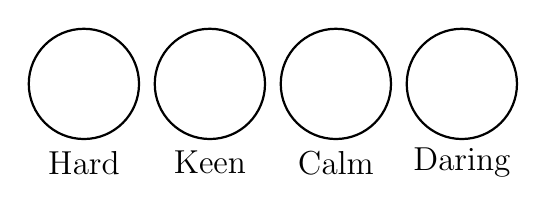
\begin{tikzpicture}
            \node [draw, thick, circle, minimum size=14mm, xshift=3mm] (h) {};
            \node [below of=h] {\large\fauxsc{Hard}};
            \node [draw, thick, circle, minimum size=14mm, right of=h, xshift=6mm] (k) {};
            \node [below of=k] {\large\fauxsc{Keen}};
            \node [draw, thick, circle, minimum size=14mm, right of=k, xshift=6mm] (c) {};
            \node [below of=c] {\large\fauxsc{Calm}};
            \node [draw, thick, circle, minimum size=14mm, right of=c, xshift=6mm] (d) {};
            \node [below of=d] {\large\fauxsc{Daring}};
        \end{tikzpicture}
    \end{multicols}
    \PlaybookRuleL

    
\begin{tikzpicture}
        \node (txt) {\Large\Kochfont Stress};
        \node [draw, thick, circle, minimum size=5mm, right of=txt] (a) {};
        \node [draw, thick, circle, minimum size=5mm, xshift=-3mm, right of=a] (b) {};
        \node [draw, thick, circle, minimum size=5mm, xshift=-3mm, right of=b] (c) {};
        \node [draw, thick, circle, minimum size=5mm, xshift=-3mm, right of=c] (d) {};
        \node [draw, fill, right of=d, xshift=15mm, minimum width=43mm, minimum height=8mm] (box) {};
        \node [draw=white, thick, circle, minimum size=5mm, xshift=-3mm, right of=d, fill=white] (e) {};
        \node [draw=white, thick, circle, minimum size=5mm, xshift=-3mm, right of=e, fill=white] (f) {};
        \node [draw=white, thick, circle, minimum size=5mm, xshift=-3mm, right of=f, fill=white] (g) {};
        \node [draw=white, thick, circle, minimum size=5mm, xshift=-3mm, right of=g, fill=white] (h) {};
        \node [draw=white, thick, circle, minimum size=5mm, xshift=-3mm, right of=h, fill=white] (i) {};
        \node [draw=white, thick, circle, minimum size=5mm, xshift=-3mm, right of=i, fill=white] (j) {};
        \node [draw=white, ultra thick, dash pattern={on 1pt off 1pt}, circle, minimum size=6mm, xshift=-3mm, right of=i] (j) {};
    \end{tikzpicture}
    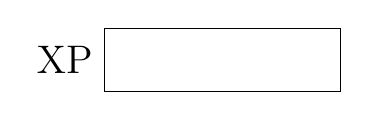
\begin{tikzpicture}
        \node (txt) {\Large\Kochfont XP};
        \node [draw, xshift=10mm, minimum width=30mm, minimum height=8mm, right of=txt] (box) {};
    \end{tikzpicture}

    \begin{multicols*}{2}
        \raggedcolumns
        \uline{\Large\Kochfont Triggers\hfill}
        \begin{itemize}
            \item If you took a life. \dotfill{}1 Stress
            \item If there was combat. \dotfill{}1 Stress
            \item If your plane got shot. \dotfill{}1 Stress
            \item If you were wounded. \dotfill{}2 Stress
            \item If a comrade was wounded. \dotfill{}2 Stress
            \item If your plane stopped working. \dotfill{}2 Stress
            \item If you had to wingwalk. \dotfill{}1 Stress
            \item If the job got out of hand. \dotfill{}2 Stress
        \end{itemize}

        \columnbreak

        \uline{\Large\Kochfont Vents\hfill}
        \begin{itemize}
            \item Complain about your circumstances to a
                  comrade.
            \item Buy something nice for yourself.
            \item Complain about pay to a comrade.
            \item Stir up trouble with the employees.
            \item Deliberately trigger End of Night by
                  maxing out your Vice track.
        \end{itemize}
    \end{multicols*}
    \PlaybookRuleL
    \begin{NiceTabular}[rules/width=0.5mm]{X|X}
        \Block{1-1}{
            \uline{\Large\Kochfont Comrades\hfill \Large\Kochfont Trust?}

            \hfill
            
\begin{tikzpicture}
                \node [draw, very thick, circle, minimum size=6mm] (a) {};
                \node [draw, very thick, circle, minimum size=6mm, yshift=0mm, below of=a] (b) {};
                \node [draw, very thick, circle, minimum size=6mm, yshift=0mm, below of=b] (c) {};
                \node [draw, very thick, circle, minimum size=6mm, yshift=0mm, below of=c] (d) {};
            \end{tikzpicture}
        } &
        \Block{1-1}{\uline{{\Large\Kochfont Familiar Vices}\hfill}

            \begin{tikzpicture}
                \node [draw=white, very thick, circle, minimum size=6mm] (a) {};
                \node [draw=white, very thick, circle, minimum size=6mm, yshift=0mm, below of=a] (b) {};
                \node [draw=white, very thick, circle, minimum size=6mm, yshift=0mm, below of=b] (c) {};
                \node [draw=white, very thick, circle, minimum size=6mm, yshift=0mm, below of=c] (d) {};
            \end{tikzpicture}
        }
    \end{NiceTabular}
    \PlaybookRuleL
    \PlaybookParagraph{Intimacy Move}{Start with this move.}

    \textbf{Share the Burden}: \textit{When you are intimate with comrades}, the Stress of all the characters
    participating can be freely redistributed between them. If there are any NPC participants, 1
    Stress is also removed from each PC.

    \textit{If you use this move in the air}, 1 additional Stress is removed from each character.
    \vfill

    \columnbreak
    \PlaybookParagraph{Personal Moves}{Take Stiff Masked and choose 3 more.}
    \begin{itemize}
        \renewcommand{\labelitemi}{{\LARGE\bullet}}
        \item \textbf{Breadwinner}: Instead of personal upkeep, you have two Dependents. Write their names,
              and mark 1 on one and 2 on the other. Each Routine, during Expenses, choose to pay 0,
              1, or 2 Thaler for each Dependent. If you pay 0, erase one mark. If you pay 2, mark their
              track and describe what special thing you do for them to make their lives easier.

              A Dependent at 2 Marks removes 1 Stress per routine. A Dependent losing a Mark gives
              1 Stress, and at 0 Marks they cause 2 Stress per routine.
    \end{itemize}
    \begin{NiceTabular}{XX}
        \begin{tikzpicture}
            \node [draw=black, thick, circle, minimum size=5mm] (a) {};
            \node [draw=black, thick, circle, minimum size=5mm, xshift=-4.5mm, right of=a] (b) {};
            \draw [line width=0.5mm] ($(a)+(-3.5mm,-2.6mm)$) -- ++(-40mm,0);
        \end{tikzpicture}
         &
        \begin{tikzpicture}
            \node [draw=black, thick, circle, minimum size=5mm] (a) {};
            \node [draw=black, thick, circle, minimum size=5mm, xshift=-4.5mm, right of=a] (b) {};
            \draw [line width=0.5mm] ($(a)+(-3.5mm,-2.6mm)$) -- ++(-40mm,0);
        \end{tikzpicture}
    \end{NiceTabular}
    \PlaybookRuleR
    \begin{itemize}
        \renewcommand{\labelitemi}{{\large\circ}}
        \item \textbf{There for You}: \textit{When you Get Real}, your target always loses 1 extra Stress.
        \item \textbf{Get it Done}: Each Routine, hold 3. Spend that hold to score a partial hit on any roll,
              without rolling first.
        \item \textbf{Time Out}: \textit{When you intervene in a dispute}, \underline{roll +Calm}. On a hit, the conflict cannot
              escalate to violence. 16+, everyone names a compromise they would be willing to make.
        \item \textbf{Hard Drinking}: You may reroll two dice in the End of Night roll.
        \item \textbf{Old Reliable}: After 3 Routines in the same plane, without it being modified or upgraded,
              the plane gains +8 Toughness and +3 Reliability. This is once per plane, and the bonus is
              removed if the plane is modified.
        \item \textbf{No Drama}: The first time each Routine that somebody Vents with you as the victim,
              instead of Stress you take 2 XP directly.
        \item \textbf{Open Mind}: \textit{When you perform a Move Exchange}, both sides can learn as many moves
              as they have XP for from one another, instead of just 1. Other playbook moves cost 1 less
              XP to learn, and this character can teach any move they’ve learned.
        \item \textbf{Domestic Bliss}: While you have 0 Stress, take +1 ongoing to all rolls outside of air combat.
    \end{itemize}
    \PlaybookRuleR
    \PlaybookParagraph{Other Moves, \& Notes}{Start with 1 Mastery Move and 3þ.}

    All your XP costs are doubled.
    \vfill

    \hfill
    \begin{tikzpicture}[overlay]
        \node [draw=black, thick, circle, minimum size=5mm, xshift=3mm, yshift=-18mm] (a) {};
        \node [draw=black, thick, circle, minimum size=5mm, xshift=4.5mm, left=5.1mm of a] (b) {};
        \node [draw=black, thick, circle, minimum size=5mm, xshift=4.5mm, left=5.1mm of b] (c) {};
        \node [draw=black, thick, circle, minimum size=5mm, xshift=4.5mm, left=5.1mm of c] (d) {};
        \node [draw=black, thick, circle, minimum size=5mm, xshift=4.5mm, left=5.1mm of d] (e) {};
        \node [xshift=4.5mm, anchor=east, left=3.8mm of e](txt) {\Large\Kochfont Mastery Progress};
    \end{tikzpicture}
}

\end{document}